% !TEX root = paper.tex
\section{Tyne and Wear ANPR Data}\label{s.ncl}

Automatic number plate recognition (ANPR) cameras are actively employed in urban traffic environments and play an important role in day-to-day intelligent transportation systems. They can be used by government subsidised entities in urban traffic management and control; by comissioned highway agencies in electronic toll collection; or by law enforcement organisations in detecting speeding vehicles and validating number plate registrations. The wide diversity of applications, paired with the large improvements in price-to-performance ratios of ANPR hardware and software systems, has resulted in increased investments of ANPR cameras for urban environments~\cite{EvolutionUTMC2013, SurveyITS2011}.

\begin{figure}[t]
\centering
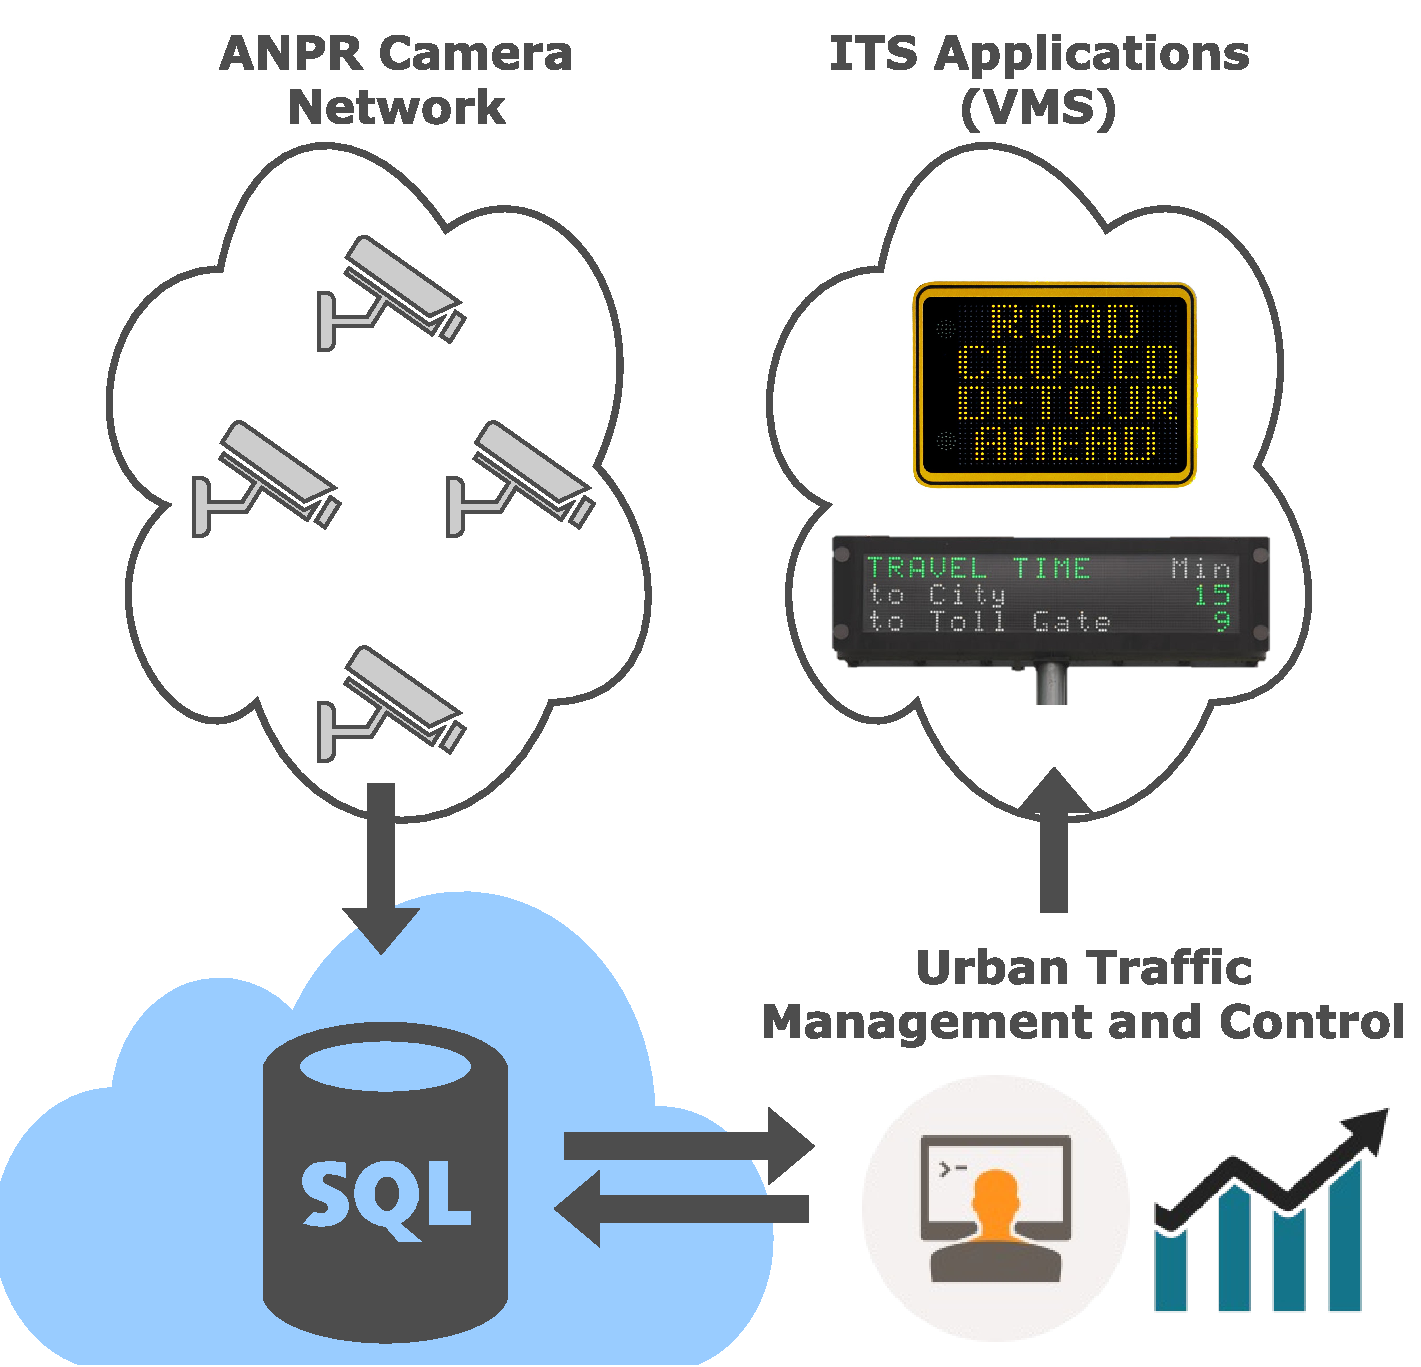
\includegraphics[width=.95\linewidth]{ANPR-overview.pdf}
\caption{}
\label{fig:anpr-overview}
\end{figure}

In the region of Tyne and Wear, United Kingdom, there are over 250 active ANPR cameras. This network of cameras records over 1 million license plate detections every day. Figure~\ref{fig:time-series} shows how the number of sightings fluctuates over a single month (February, 2017). Furtheremore, scans made by these cameras are stored in a central database by the Urban Traffic Management and Control (UTMC) of Tyne and Wear and are then used to compute travel times across particular links of interest in the road network. These are usually major roads that see high volumes of traffic, or road segments more prone to traffic jams. Average journey times can then be conveyed back to the drivers by the way of Variable Message Signs (VMS) or web based applications. Figure~\ref{fig:anpr-overview} represents this interaction.

\begin{figure*}[t]
\centering
\begin{subfigure}[t]{.48\textwidth}
  \centering
  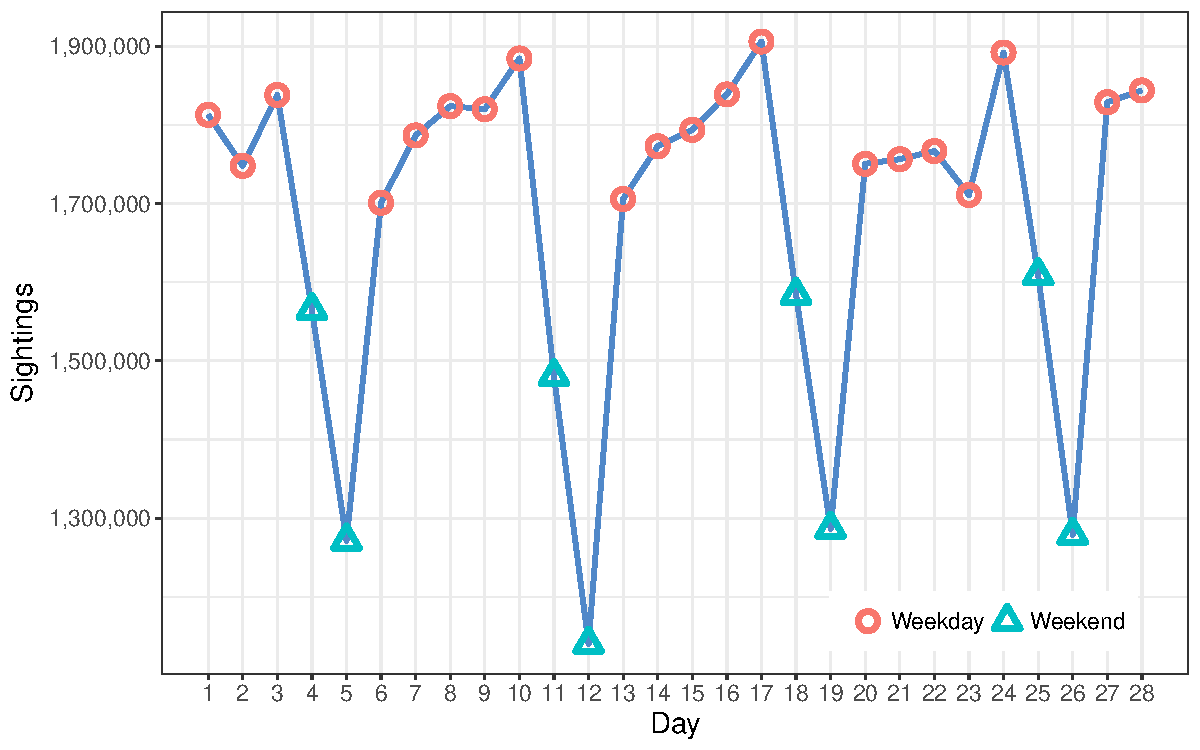
\includegraphics[width=.9\linewidth]{observations_per_day.pdf}
  \caption{Total number of scans recorded per day in Tyne and Wear. There is a clear seasonal effect caused by decreasing traffic demands in weekends and increasing traffic volume in weekdays.}
  \label{fig:observations-per-day}
\end{subfigure}\hfill
\begin{subfigure}[t]{.48\textwidth}
  \centering
  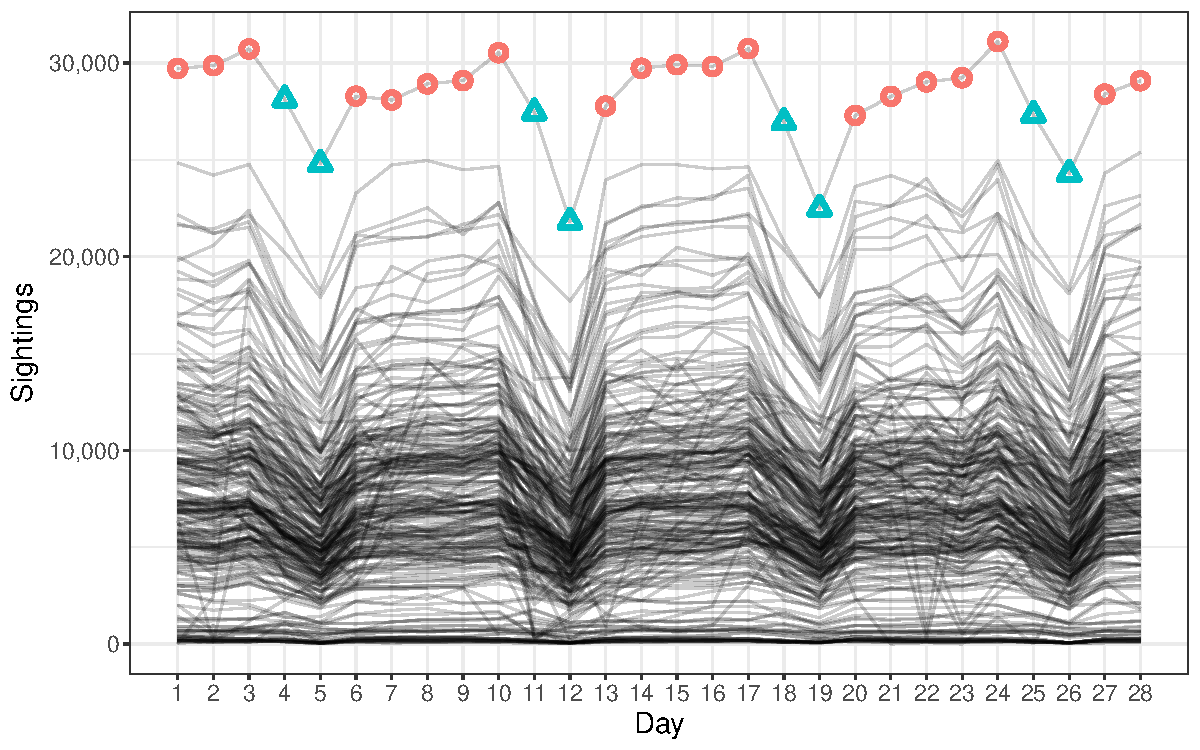
\includegraphics[width=.9\linewidth]{observations_per_day_camera.pdf}
  \caption{Number of scans recorded per ANPR camera and day in Tyne and Wear. Inter-camera variability is observed, as some cameras are located in more traffic intensive road sections than others. Decomissioned or temporarily unavailable cameras (due to loss of power, faulty camera, road closed, etc) are depicted at the bottom of the graph.}
  \label{fig:observations-per-camera-day}
\end{subfigure}
\caption{License plate scans recorded by ANPR cameras during February 2017, in the region of Tyne and Wear, United Kingdom.}
\label{fig:time-series}
\end{figure*}
